\chapter{Conclusions and future work}
In this chapter we will review what was expected to be done by the end of the final project, what has finally been done and how. Also
we will talk about what was expected and has yet to be done, and ideas that came during the development process but can not be implemented
because of the lack of time.
\section{Goals review}
% TODO Make a revision of all the goals exposed on this document as an intention,
% 	and explain what is the result, why is this way and what have to be improved.
Our goal at the beginning of this final project was to develop an event-driven job scheduler which could receive multiple kinds of events.
Those jobs would shell commands because we want them to be general purpose.
Its main feature would be that the execution of the jobs is state-aware, so it would run state machines that define the scheduling.
This would permit us to control situations like ``Execute 'x' if we haven't executed it yet''. Also we wanted a client that resent events
detected in the machine in which it is running to a server machine that could react to them.\\
Those goals are pretty much achieved. Our software is centred in a daemon which computes state machines. An state machine is a set of 
states connected by transitions. We go from one state to another by a transition when we receive a set of events specified in 
every transition. Also, when we change of state using a transition, this one may execute an action. In our case, the 
events of the transitions are the events that run jobs, and the transition actions are the jobs. So we transformed the job scheduling
rule-making to an state machine definition. That makes the project an state-aware and event-driven job scheduler, so this point is solved too.\\
The version we release for this final project can receive several kinds of events, thanks to the command-line control program that can send
events to the daemon. It permits to receive events from existing job-schedulers of different kinds such as \emph{cron}, \emph{syslog} or
\emph{udev}. But also we have two sources of events more that makes our project \emph{potentially} able to receive lots of different kinds
of events. This is the event-sending library and the plugin workers, which need some minimal development.\\
Our state machines can execute several kinds of actions like shell commands. Another kind of actions that we have is the 'propagate' 
action. Those actions, as we have seen, propagates all the events that triggered itself, so it achieves the client/server model goal.
\section{Future work}
\label{sec:future}
There are features that we expected to have for this final project that finally we had no time to implement. Some of those does not
have a design because it was intended to be done on a future development iteration. However, those features had low priority because
they are not very related to the main goals of the project.\\
Other features were thought later, when the design and the planning were already defined so we had no time left to make them real.\\
We also have work to be done related to design improvements and bug-fixing.\\
This future work is divided into two categories, critical and new features. In critical will be bug-fixing and design changes. New features
are just that, features that will make the software better and more useful.
% TODO Explain the solution to the 'others' logout problem.
\subsection{Critical}
\subsubsection{Log \texttt{CMD} actions output}
We have to design and implement a way to monitor the \texttt{CMD} actions and get the strings it tries to print in the standard output, in
order to log them. For example, if we execute a command, it fails and writes the error information in the standard output, the user would
want to know what this message said.\\
To do that we probably will need to make a thread that reads a pipe to the command programs.
\subsubsection{Non-connex cycle component}
We explained in \emph{section \ref{sec:smman}} that when we remove a transition that is followed by a cycle, the cycle won't be removed and
won't be connex to the beginning of the state machine. This is a problem to solve by using a BFS algorithm to check the connectivity of the
state machine every time we remove a transition and it doesn't remove the destination state.
\subsubsection{User credential control}
In \emph{section \ref{sec:users}} we describe the design of the user credential control system of \emph{reactor}. To summarize, we have
three levels of users and the lower lever users can not reach the resources of the higher level users. This resources are mainly the state 
machines and the way to reach them are through control commands and events.\\
The implementation of this system has to be done yet, and the design of the remote events credential control system has to be detailed a
lot more.
\subsubsection{Graphical state machine visualization}
The idea is 
to be able to generate a representation of the state machines we have loaded in a known format. This way it can be passed to a graph
rendering program in order to visualize it. For example there is the DOT\cite{graphviz:dot} language, which is pretty popular and is used
by the also popular \emph{Graphviz}\cite{graphviz} project.\\
This would let the user get a lot of useful information about the state machines running on \emph{reactord}, like the current states or
the identifier numbers of the transitions.
\subsubsection{Current state storing}
It can be seen in the planning (\emph{\ref{sec:tasks}}), but it doesn't appears neither in the specification nor in the design of the 
project, because of the lack of time. What we want is to allow the user select states to make them able to be saved. This means that when
the daemon stops it will save that it was stopped in this state. When the daemon is started again it will put as current states the ones 
saved, instead of the initial states.\\
One way of mark these states would be using the key character \texttt{*}. i.e.:
\begin{center}
  \texttt{STATE\_A STATE\_B* e1 \& e2 NONE}
\end{center}
If the state machine that contains that transition is in \texttt{STATE\_B} when \emph{reactord} is stopped, then this would be saved, and
the next time \emph{reactord} starts the state machine will began in \texttt{STATE\_B} instead of its initial state. However if this 
happens in \texttt{STATE\_A} nothing will be saved and in a posible \emph{reactord} restart the state machine would begin normally
at the initial state.
\subsubsection{Performance analysis}
This is probably the most important work to be done. It was planned to be performed by the last deadline of the project, but the final lack
of time did not allow us to do it.\\
This is not a new feature or a bug-fix by itself, but it will help us to detect the bottlenecks of \emph{reactor} and find solutions. It 
is critical because our project is based on a daemon running with root permissions that could be performing a lot of actions and have lots
of huge state machines. It is important to push \emph{reactor} to the limit and measure its behaviour.\\
By the theory we can sense that removing a transition from a huge state machine would be very costly, as it would be to put a new initial
state. Also, going forward from a state with a lot of leaving transitions would be slow.\\
But that's all we have by now, theory and speculation and we need to solve this in order to improve our project.
\subsection{New features}
Future useful features for our project.
\subsubsection{Empty set of events}
As we will see later in \emph{\ref{sec:smcom}}, there are situations in which we would like to have an empty set of events in order to run
an action and go to the next state. For this we will define the symbol \texttt{-}, which will mean empty event set. The transitions
with this symbol as a set of events will be executed when we arrive to its leaving state.
\subsubsection{State machine intercommunication}
\label{sec:smcom}
By now we do not plan to make \emph{reactord} able to join different state machines with a transition, because as we said, it results
a very complex software design and it doesn't provide really important features.\\
But there is another kind of state machine intercommunication much more useful and easy to develop. We are
talking about making a transition able to ask if we are in a concrete state that could be from another state machine.\\
Right now, when we are executing the action of a transition, we do it because we received some events when we were in a
concrete state in its state machine. The idea is to extend this to check states of other state machines when we receive an event in order 
to go forward. \emph{Figure \ref{fig:smcom}} is an example of this.
\begin{figure}[h]
  \centering
  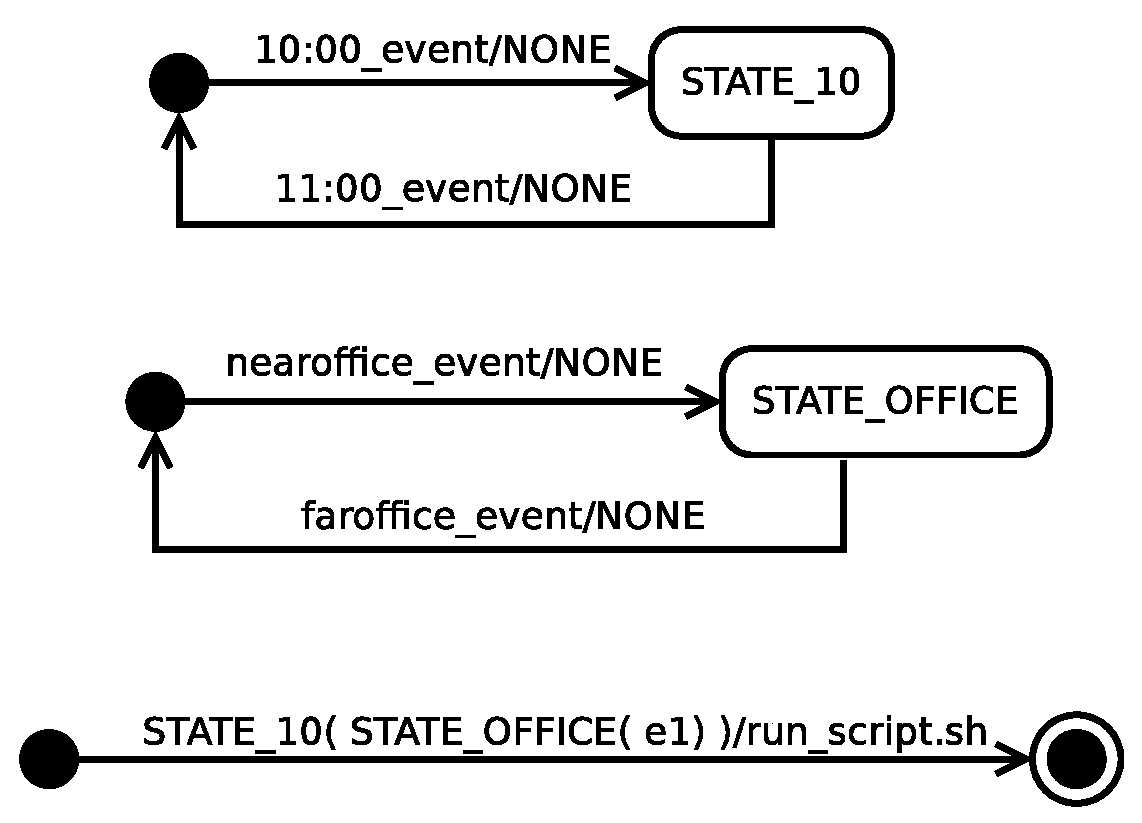
\includegraphics[width=0.7\textwidth,keepaspectratio]{img/smcom}
  \caption{A state machine making use of the intercommunication feature}
  \label{fig:smcom}
\end{figure}
In the last state machines only transition, where the events are supposed to be, we have ``\texttt{STATE\_10( STATE\_OFFICE( e1 ) )}''.
\texttt{STATE\_10} and \texttt{STATE\_OFFICE} are states from the other state machines. The way to read this is ``if we receive \texttt{e1}
while we are in state \texttt{STATE\_OFFICE} and while we are in state \texttt{STATE\_10}, then run the action and go to the next state''.
That makes us able to have independent state machines doing nothing more than controlling states in the daemon, useful for other 
more functional state machines.\\
We could have the events field look like ``\texttt{STATE\_10( STATE\_OFFICE( - ) )}'', so we don't wait for any event, but to the state 
machines to be in those states at the same time.\\
We could make it also able to ask for states in remote machines.
\subsubsection{Extend plugins interface}
The easiest way to add new features to \emph{reactor} is to extend the plugins interface. To be precise, we have two extensions in mind:
\begin{itemize}
  \item {\bf Black-box states}\\
    The ability to ask to the plugins if we are in a specific state, like in \emph{section \ref{sec:smcom}}. The difference is that the
    user or \emph{reactord} knows nothing about the supposed state machine in which the asked state is. We can ask if we are in the 
    ``between 10:00AM and 11:00AM'' state, but we don't know how this is controlled. Probably the plugin will just ask to the system clock,
    which makes much more sense than having to control it all the time with our state machine.
  \item {\bf Parser accessible to \emph{reactord}}\\
    Having the \emph{reactord} rules in one file and then the plugins rules in several files can become a mess. One way to solve that is to
    use as event identifier in the \emph{reactord} rules the plugin rule that triggers the event. i.e:
    \begin{center}
      \texttt{STATE\_A STATE\_B @cron:``0 1 * * *'' CMD script.sh}
    \end{center}
    The only event in this rule is \texttt{@cron:``0 1 * * *''}. \texttt{@cron:} identifies the plugin and what is between \texttt{``} and
    \texttt{''} is a rule of the the 'cron' plugin.\\
    Internally those rules would be loaded by the plugin when \emph{reactord} starts and would make a hash-like identifier for it.
\end{itemize}
\subsubsection{User monitor plugin}
This feature would not be a \emph{reactor} internal, but a useful plugin for the system administrator. As it is explained on this 
documentation, the lowest privileged \emph{reactor} users have to load their state machines manually, so they need to login in the system 
in order to make use of \emph{reactor}. The problem is that when they logout their state machines will be running and maybe this is 
something the system administrator doesn't want. To solve this we can make a plugin to notice users login and logout events.
This way the system
administrator can make a state machine waiting for user monitoring events to remove the state machines of other users once they logout.
\subsubsection{\texttt{CMD} action finish events}
A \texttt{CMD} action finishing and its return value is a source of events very useful for our system. It is so because we can make
an state machine wait in a state until an action finishes with it. And also we can continue with a different flow depending on if the
command returned 'success' or 'fail. In \emph{figure \ref{fig:actionevents}} we have a simple example of it.
\begin{figure}[h]
  \centering
  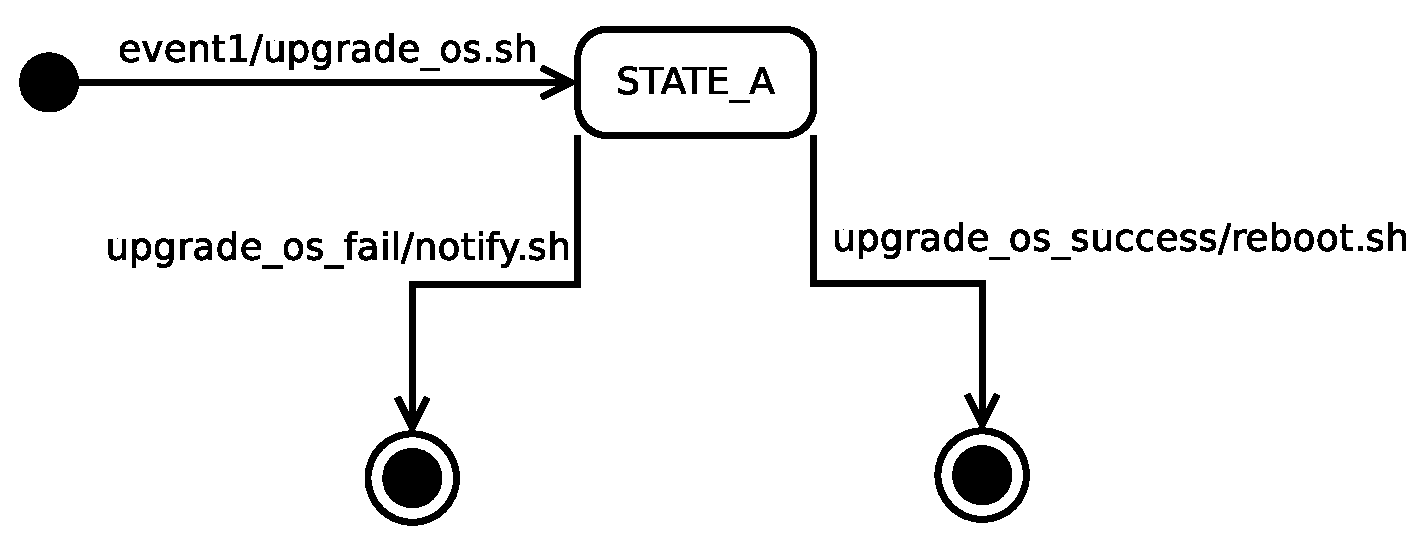
\includegraphics[width=0.7\textwidth,keepaspectratio]{img/actionevents}
  \caption{A state machine making use of the \texttt{CMD} action finish events.}
  \label{fig:actionevents}
\end{figure}
With the first transition it upgrades de system. It waits until the process is finished and, if everything went fine, then reboots the 
system. If not it notifies the user.
% \section{Personal conclusions}
% The impact of this project on me can be summarized in one phrase: I learned a lot, really. This is project was new for me from several 
% points of view.\\
% This is my first personal long-term project. It is the first time that I specify, design and implement all by myself a project like this,
% in a infinite iteration development process.\\
% It is 